\section{Introduction}\label{sec:intro}

Electricity systems are managed through many local decision units that commit resources before uncertainty resolves.
Every day, each of the balancing authorities, national system operators and regional market operators that run the world's grids must commit enough capacity to meet the next day's hourly demand.
Committing too little forces expensive real-time purchases, the activation of reserves or, in the worst case, load shedding; committing too much means paying for capacity that sits idle.
The cost of a shortfall is not the same everywhere: an operator embedded in a dense web of interconnections can import from its neighbours, while an isolated system cannot.
Winter Storm Uri in February 2021 is the extreme example: failures of frozen generators and gas supply forced the weakly interconnected Texas grid to shed load for days, and its limited ability to import deepened the crisis, while neighbouring systems with more import capability shed much less \citep{Busby2021,FERCNERC2021}.
At the same time, governments are committing to large battery-storage programmes, and planners must decide where those batteries should go.

Operators and planners do not lack forecasts.
Operators publish their own day-ahead forecasts, simple persistence and calendar rules are always available, statistical and machine-learning models can be trained on the data, and pretrained foundation models now forecast any series zero-shot \citep{Ansari2024chronos}.
None dominates everywhere, which makes combining them attractive.
How to combine them is less obvious.
The forecast-combination and model-averaging literature, from \citet{BatesGranger1969} to the asymptotic theory of \citet{Hansen2007}, \citet{HansenRacine2012}, \citet{ZhangWanZou2013} and \citet{ZhangLiu2023}, offers two options when there are many series.
Weights can be estimated series by series, which respects heterogeneity but produces noisy weights when histories are short---the root of the ``forecast-combination puzzle'' that simple averages often beat estimated weights \citep{SmithWallis2009,Claeskens2016}.
Or one set of weights can be estimated for all series, which is precise but imposes the same rule on systems that face different conditions.
Deep learning offers a third option, a network that maps features to weights \citep{MonteroManso2020,Gong2026moe}, at the price of thousands of parameters and weights that are hard to audit.
All three typically judge a combination by its statistical accuracy, although the planner is judged by the cost of the resulting decisions; the decision-focused literature in operations management has shown that learning directly for the decision can be much better than forecasting accurately and then optimising \citep{BanRudin2019,BertsimasKallus2020,ElmachtoubGrigas2022}.

This paper proposes \emph{grouped decision-focused model averaging} (GDMA) and uses it to answer three management questions: how should grid operators on five continents combine the forecasts they have into day-ahead capacity commitments, who gains and who loses from a common planning rule, and where should new batteries be installed?
GDMA assumes that decision units fall into a small number of latent segments whose members are best served by the same combination of candidate rules, and estimates the segments and the segment-specific weights jointly by minimising the realised system-wide decision cost, in money, with each unit's own cost asymmetry.
A soft version shrinks each unit's own weights towards those of its segment.
The number of segments and the shrinkage intensity are chosen by a time-ordered hold-out.
Pooled weights, unit-specific weights and shrinkage towards pooled weights are special cases, and the combined commitment is always a convex combination of commitments the operator already understands.
A second, planning stage takes the residual shortfall risk left by the learned rule and allocates a storage budget across grid areas.

\begin{figure}[t]
\centering
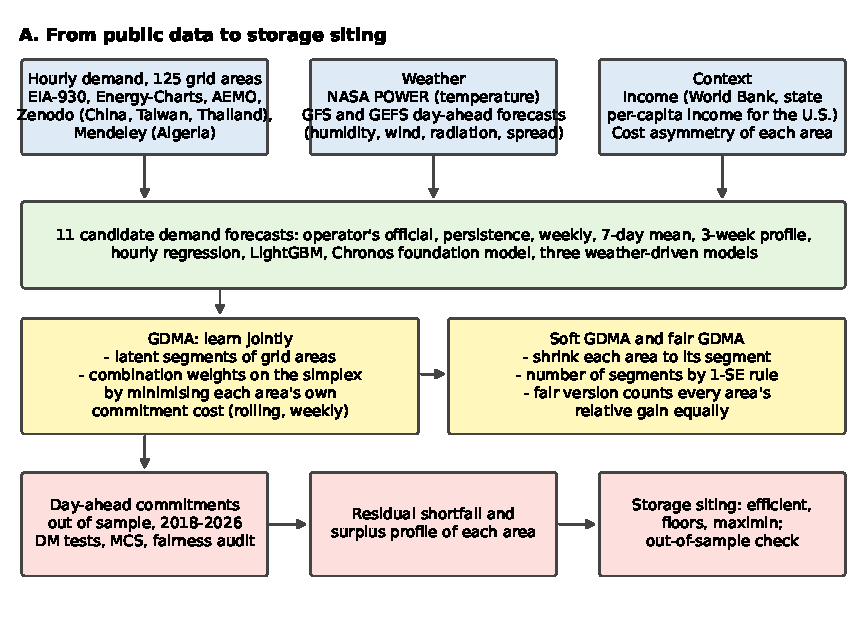
\includegraphics[width=0.9\textwidth]{figures/fig_pipeline.pdf}
\caption{The approach from public data to storage siting.}\label{fig:pipeline}
\end{figure}

\begin{figure}[t]
\centering
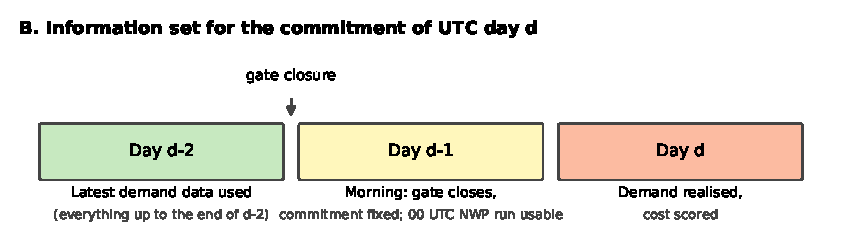
\includegraphics[width=0.95\textwidth]{figures/fig_timeline.pdf}
\caption{Information set of the day-ahead commitment. Data up to the end of day $d-2$ and the 00~UTC weather forecast of day $d-1$ (only where it is available before gate closure) enter the commitment for day $d$.}\label{fig:timeline}
\end{figure}

Figure~\ref{fig:pipeline} summarises the approach and Figure~\ref{fig:timeline} the timing of the information.

We make five contributions.
\begin{enumerate}
\item \textbf{Method.} We formulate the joint learning of latent segments and combination weights under an asymmetric, unit-specific decision loss, give a $k$-means-type algorithm with regret-space seeding in which every step is a small convex program, and link it to a storage-siting problem that is solved exactly by a greedy algorithm (Section~\ref{sec:method}).
To our knowledge, neither the model-averaging, the decision-focused learning nor the latent-group panel literature \citep{BonhommeManresa2015,Su2016} has proposed this estimator.
\item \textbf{Learning theory.} We prove a finite-sample oracle inequality that separates the cost of learning memberships ($\log G/T$ per unit) from the cost of learning weights ($GM\log(NT)/(NT)$), which shows how the cost of grouping scales relative to unit-specific weights when histories are short; we show that GDMA is asymptotically optimal and, under a segment structure, attains the risk of the infeasible benchmark in which every unit knows its own optimal weights; that it recovers the segments with probability approaching one; and that on this event it coincides exactly with an estimator told the segments (Section~\ref{sec:theory}).
\item \textbf{Evidence on five continents.} We evaluate all rules with the information available at the day-ahead gate closure. On 46 U.S.\ balancing authorities with their official forecasts (Section~\ref{sec:app}) and on a global panel of 125 grid areas in North America, Europe, Oceania, Asia and Africa (Section~\ref{sec:global}), soft GDMA lowers the stylised out-of-sample commitment cost by 13--17\% relative to the official forecasts in the United States and by 12\% worldwide relative to a reference forecaster, beats combining the same forecasts for accuracy by 2--3 points in the United States (at $W=28$) and 8--10 points worldwide, and beats a decision-focused neural mixture-of-experts gate by seven percentage points worldwide. Decision-focused shrinkage and two-step clustering come close, and a model confidence set cannot separate the grouped variants from one another, so the evidence is for decision-focused combination with cross-sectional structure rather than for grouping alone. A pretrained foundation model and models driven by archived day-ahead deterministic and ensemble weather forecasts enter the candidate set on equal terms; the ensemble information roughly halves, but does not close, the gap to the operators' own forecasts during Winter Storm Elliott, the most abrupt event in the sample.
\item \textbf{Fairness.} We audit how the gains are distributed across grid areas and propose a fair variant that counts every area's relative improvement equally. Soft GDMA makes 6\% of areas worse off than their own best candidate, against 24\% for pooled weights and 42\% for the neural gate, shows no systematic gradient with national or state income that the data can detect, and its fair variant halves the share of areas made worse off at no cost in total (Section~\ref{sec:fairaudit}).
\item \textbf{Storage siting.} In a stylised storage model, better commitment rules reduce what storage can add: the reference rule needs 34\,GW of optimally sited batteries to reach the cost that soft GDMA achieves without any. The optimal location of a storage programme depends on the commitment rule, but siting on the wrong rule's error profile loses only 2--4\% of a programme's value, and maximin-fair siting helps the worst-served continent at a price of fairness of 7--9\% (Section~\ref{sec:storage}).
\end{enumerate}

The paper speaks to the theme of this special issue in both directions it describes: it develops a statistical learning method with guarantees, motivated by a concrete management problem, and it uses new, openly available data and models to answer a planning question of continental scale.
Replication code and data-construction scripts are available in a public repository (see the data availability statement).
